%%% License: Creative Commons Attribution Share Alike 4.0 (see https://creativecommons.org/licenses/by-sa/4.0/)


%%%%%%%%%%%%%%%%%%%%%%%%%%%%%%%%%%%%%%%%%

%----------------------------------------------------------------------------------------
%	PACKAGES AND OTHER DOCUMENT CONFIGURATIONS
%----------------------------------------------------------------------------------------

\documentclass[a4paper]{article}

\usepackage{amssymb}
%\usepackage{enumerate}
\usepackage[usenames,dvipsnames]{color}
\usepackage{fancyhdr} % Required for custom headers
\usepackage{lastpage} % Required to determine the last page for the footer
\usepackage{extramarks} % Required for headers and footers
\usepackage[usenames,dvipsnames]{color} % Required for custom colors
\usepackage{graphicx} % Required to insert images
\usepackage{listings} % Required for insertion of code
\usepackage{courier} % Required for the courier font
\usepackage[table]{xcolor}
\usepackage{amsfonts,amsmath,amsthm,parskip,setspace}
\usepackage[section]{placeins}
\usepackage[a4paper]{geometry}
\usepackage[USenglish]{babel}
\usepackage[utf8]{inputenc}
\usepackage{tikz}
\usepackage{hyperref}
\usepackage[hyphenbreaks]{breakurl}
\usepackage[]{url}
\usepackage{enumitem}


% Margins
\topmargin=-0.45in
\evensidemargin=0in
\oddsidemargin=0in
\textwidth=6.5in
\textheight=9.0in
\headsep=0.6in

\linespread{1.1} % Line spacing



%----------------------------------------------------------------------------------------
%   FORMATTING
%----------------------------------------------------------------------------------------
% Set up the header and footer
\pagestyle{fancy}
\lhead[c]{\textbf{{\color[rgb]{.5,0,0} K{\o}benhavns\\Universitet }}} % Top left header
\chead{\textbf{{\color[rgb]{.5,0,0} \Class }}\\ \hmwkTitle  } % Top center head
\rhead{\instructor \\ \theprofessor} % Top right header
\lfoot{\lastxmark} % Bottom left footer
\cfoot{} % Bottom center footer
\rfoot{Page\ \thepage\ of\ \protect\pageref{LastPage}} % Bottom right footer
\renewcommand\headrulewidth{0.4pt} % Size of the header rule
\renewcommand\footrulewidth{0.4pt} % Size of the footer rule


% Other formatting stuff
%\setlength\parindent{12pt}
\setlength{\parskip}{5 pt}
%\theoremstyle{definition} \newtheorem{ex}{\textbf{\Large{Exercise & #}\\}}
\usepackage{titlesec}
\titleformat{\section}[hang]{\normalfont\bfseries\Large}{Problem \thesection:}{0.5em}{}




%----------------------------------------------------------------------------------------
%	NAME AND CLASS SECTION
%----------------------------------------------------------------------------------------
\newcommand{\hmwkTitle}{Midterm} % Assignment title
\newcommand{\Class}{Mechanism Design} % Course/class
\newcommand{\instructor}{Fall 2024} % TA
\newcommand{\theprofessor}{Prof. Egor Starkov} % Professor




%----------------------------------------------------------------------------------------
%   SOLUTIONS
%----------------------------------------------------------------------------------------
\newif\ifsolutions
\solutionstrue




\begin{document}
	
	\begin{center}
		\LARGE\textbf{Midterm assignment}
	\end{center}
	
	
	Be prepared that the problems below can be more messy and/or difficult than the problem sets.
	Group submissions are allowed and encouraged (no more than 5 people per group). If something in the assignment is ambiguous or you think something is incorrect, email me.
	
	
	
	
	\section{(Malevolent) Judicial design}
	%old Jeff's problem bank
	%solo IC
	
	A suspect is in custody, accused of murder.  If he goes to trial he will either be convicted or acquitted. If he is convicted he will be sent to prison for life giving him a payoff of $-1$.  If he is acquitted he goes free and has a payoff of $0$.  The district attorney can offer plea bargains: allowing the defendant to plead guilty in return for a lighter sentence.  In particular, for any $r\in (0,1)$, the DA can offer a reduced sentence which, if accepted, would give the defendant a payoff of $-r.$
	
	The defendant is privately informed about his chances for acquittal at trial:  $\theta\in [0,1]$ is the defendant's privately known probability of acquittal.  If the defendant does not enter into a plea bargain with the DA he will go to trial and be convicted with probability $1 - \theta$.
	
	Consider the mechanism design problem where the DA is the principal and the defendant is the agent.  A social choice function is a mapping $f:[0,1] \rightarrow \left\{ \text{trial} \right\} \cup (0,1)$ where $f(\theta) = \text{trial}$ means that type $\theta$ will go to trial and $f(\theta) = r \in (0,1)$ means that type $\theta$ accepts a plea bargain giving him a sentence with payoff $-r$. DA thinks $\theta$ has full support on $[0,1]$.
	
	\begin{enumerate}
		\item Write down the inequalities that characterize whether some given social choice function $f$ is incentive-compatible	for the defendant.
		\item What is the set of all incentive-compatible social choice functions?
		You can proceed in the following steps:
		\begin{itemize}
			\item Show that in any IC $f$ at most one plea bargain $r$ is available.
			\item Show that $f$ must be of cutoff type, with the suspect taking the plea if $\theta < \bar{\theta}$ and going to court otherwise.
			\item Find the value of $r$ that makes the cutoff s.c.f. $f$ incentive compatible given some cutoff type $\bar{\theta}$.
			\item Combine all of the above to characterize the set of implementable $f$.
		\end{itemize}
	\end{enumerate}
	
	Suppose that the DA wants to maximize the expected length of the defendant's sentence, i.e. to minimize the defendant's expected payoff. (So the DA gets a payoff of $1$ for a life sentence and a payoff of $r$ for a reduced sentence which would give the defendant a payoff of $-r$.)  
	\begin{enumerate}[resume]
		\item Among the incentive-compatible mechanisms you identified, what is the optimal mechanism for the DA?
		\item How does your answer change if going to trial imposes additional cost $c \in (0,1)$ on the DA (but not on the defendant) relative to agreeing on a plea bargain?
	\end{enumerate}
	
	
	\ifsolutions
	\subsection*{Solution}
	\begin{enumerate}
		\item By going to trial a defendant of type $\theta$ receives (expected) utility of $-(1-\theta)$, while from accepting a plea bargain his utility is $-r$. 
		%This implies that the IC constraint is $f(\theta)=r \Rightarrow -r\geq -(1-\theta) ~\&~ \forall \theta' \neq \theta ~ f(\theta') \geq f(\theta)$.
		Fix some s.c.f. $f(\theta)$. Let $\Theta_p$ be the set of types who are offered a plea bargain $f(\theta) = r(\theta)$, and $\Theta_t$ be the set of types who are meant to go to trial: $f(\theta) = \text{trial}$ ($\Theta_t \cup \Theta_p = [0,1]$). Then the IC constraints are given by:
		\begin{align*}
			\text{ for all } \theta \in \Theta_p: \quad&-r(\theta) \geq -r(\theta') \text{ for all } \theta' \in \Theta_p
			\\
			& \text{and}  -r(\theta) \geq -(1-\theta);
			\\
			\text{ for all } \theta \in \Theta_t: \quad& -(1-\theta) \geq -r(\theta') \text{ for all } \theta' \in \Theta_p.
		\end{align*}
		
		
		\item We will characterize the set of IC social choice functions by a series of claims. 
		%For simplicity we will initially assume that $\theta$ has full support on $[0,1]$, and then correct for other cases.
		
		\begin{itemize}
			\item[claim 1] $f(\bullet)$ has at most one value on the real line.
			
			Proof: if $f(\theta_1)<f(\theta_2) ~\theta_1,\theta_2 \in [0,1]$ then a defendant of type $\theta_2$ gains higher utility by declaring $\theta_1$ (as $-f(\theta_1)>-f(\theta_2)$. This implies the mechanism is not IC for $\theta_2$.
			
			\item[claim 2] $f(\bullet)$ has a cutoff at some $\bar{\theta}$. i.e. $f(\theta)= \begin{cases} r & \text{if } \theta<\bar{\theta}
				\\
				T & \text{if } \theta\geq\bar{\theta} \end{cases}$ (value at $\bar{\theta}$ is not unique)\\
			
			Proof: assume $\theta'>\theta , f(\theta)=T, f(\theta')=r$. By IC for $\theta$ we know that $-r\leq -(1-\theta)$. However as $-(1-\theta')>-(1-\theta)$ this implies that $-(1-\theta')>-r$ and we don't have IC for $\theta'$.
			
			\item[claim 3] $u(-f(\bar{\theta}),\bar{\theta})\geq -(1-\bar{\theta})$
			
			This follows immediately from IC for type $\bar{\theta}$.
			
			\item[claim 4] $r= 1-\bar{\theta}$
			
			Proof: $r\leq 1-\bar{\theta}$ follows directly from the last claim, while $r\geq 1-\bar{\theta}$ follows from IC of type $\bar{\theta}+\epsilon$. If type $\bar{\theta}$ were strictly better of by accepting the plea bargain, by continuity and monotonicity of benefit of trial, type $\bar{\theta}+\epsilon$ would also strictly prefer the plea bargain contradicting IC for that type.
		\end{itemize}
		
		These four claims  imply that for any $(r,\bar{\theta})$ s.t. $r= 1-\bar{\theta}$ the social choice function
		
		\[ f(\theta)= \begin{cases} r & \text{if } \theta<\bar{\theta} \\
			
			T & \text{if } \theta\geq\bar{\theta} \end{cases} \]
		
		is incentive compatible.
		
		%As long as the support of types has measure one, the arguments above hold. However, if there is a interval $(a,b)$ with a zero probability, then when we set $\bar{\theta}=a$ any $r\in [a-(b-a),a]$ can be used. This is the case as claim four no longer holds, and we just need to get IC for type $b$. The same argument also holds for closed or half closed intervals.
		
		
		\item The implementable social choice functions must look as follows, for some $\bar{\theta} \in [0,1]$ (see the original problem):
		\[ f(\theta)= \begin{cases} r & \text{if } \theta<\bar{\theta} \\
			T & \text{if } \theta\geq\bar{\theta} \end{cases}, \]
		where plea bargain $r= 1-\bar{\theta}$ is offered, and the defendant can choose between that and going to trial. 
		%Note that even if the distribution does not have full support, this inly allows the DA to offer lower sentences in a plea bargain so we can ignore that case.	
		The DA gets $r$ from a plea deal and $1-\theta$ if the defendant goes to trial, so the DA's expected payoff from any such $f(\theta)$ is:
		\begin{equation}
			\label{eq:MJD}
			\begin{aligned}
				\Phi(\bar{\theta}) \cdot (1-\bar{\theta})+\int_{\bar{\theta}}^1 (1-\theta-c) d\Phi(\theta)
				&= \bar{\theta} (1-\bar{\theta}) + \frac{1-2\bar{\theta}+\bar{\theta}^2}{2} - c(1-\bar{\theta}) 
				\\&= (1-\bar{\theta}) \left(\frac{1+\bar{\theta}}{2} - c\right)
			\end{aligned}
		\end{equation}
		
		We could maximize \eqref{eq:MJD} over $\bar{\theta}$ directly. However, for $c=0$ there is a more direct solution. Any defendant who takes the the plea bargain gets a lower sentence from the plea bargain than what they would have gotten from trial. Thus, it is clearly optimal for the DA not to offer any plea bargains (except perhaps to $\theta=0$, which will accept a plea bargain of 1), i.e., setting $\bar{\theta}=0$ is optimal.
		
		\item When going to trial imposes cost $c>0$ on the DA, maximizing \eqref{eq:MJD} w.r.t. $\bar{\theta}$ yields the optimal threshold $\bar{\theta}=c$. So in the optimal mechanism, a plea deal $r=1-c$ is offered, sufficiently innocent types $\theta \in [0,c]$ take it, and types $\theta \in (c,1]$ prefer to go to trial.
	\end{enumerate}
	\fi
	
	
	
	\section{Piece of cake}
	% final2021_1. VCG, not too difficult but pretty messy
	
	Young siblings Annie and Billy are fighting over a cake of size $1$. Their respective valuations are given by $\theta_A \geq 0$ and $\theta_B \geq 0$ per unit of cake respectively and are their private information. Both kids act in pure self-interest. Their Dad decides to employ the VCG mechanism to resolve the fight.\footnote{Mom, on the other hand, prefers a Vickrey-Clarke-Groves-Weinersmith mechanism: \url{https://www.smbc-comics.com/comic/mechanism}.} 
	However, he also has preference for splitting the cake equally among the two kids: his (real) utility function is given by $v_0(k) = -\alpha(k_A - k_B)^2$, where $k_i$ is the share of the cake allocated to kid $i=A,B$.
	
	\begin{enumerate}
		\item Write down the social welfare function that is maximized by the efficient allocation $k^*(\theta)$. Explain the meaning of the parameter $\alpha$. Derive $k^*(\theta)$. 
		
		\item Derive the VCG transfers and describe the whole mechanism. (If you cannot derive the mechanism for the general case, assume $\theta_i \in [0,1]$, $\alpha > 1/4$, and derive the mechanism for this special case.)
		
		\item Since the kids are unlikely to have any money, what instrument can Dad use as transfers?
		
		%\item The VCG mechanism maximizes the social welfare, but it may cost a lot in terms of transfers. Is this an issue in this problem? If yes, what would be a better mechanism to use here? (You do not need to fully derive the alternative mechanism, just describe how you would approach the problem.)
		%%TODO: ^ clarify "cost a lot" means cost to the principal
		%TODO: the point above is vague, but also kinda weird since VCG runs a surplus
	\end{enumerate}
	
	
	
	\ifsolutions
	\subsection*{Solution}
	\begin{enumerate}
		\item The kids' real utilities are standard Euclidean, $v_i(k,\theta) = \theta_i k_i$, so the social welfare is given by 
		\begin{align*}
			w(k,\theta) = \sum_{i \in \{0,A,B\}} v_i(k,\theta) = -\alpha(k_A - k_B)^2 + \theta_A k_A + \theta_B k_B.
		\end{align*}
		Since this is effectively Dad's objective function as a designer (as opposed to $v_0$), $\alpha$ describes the weight he puts on equity relative to the kids' utilities. The efficient allocation that maximizes $w(k,\theta)$ subject to the constraint $k_A+k_B \leq 1$ is given by $k^*(\theta)=(k^*_A(\theta),k^*_B(\theta))$ with $k^*_A(\theta) = \min \left\{ \max \left\{ \frac{1}{2} + \frac{\theta_A - \theta_B}{8 \alpha}, 0 \right\}, 1 \right\}$  and $k^*_B(\theta) = 1 - k^*_A(\theta)$. 
		
		\item First we need to calculate the efficient-excluding-$i$ allocations for $i=A,B$:
		\begin{align*}
			k^{-i}_i(\theta) &= \arg \max_k \left\{ -\alpha(k_j - k_i)^2 + \theta_j k_j \right\}
			\\
			&= \min \left\{ \max \left\{ \frac{1}{2} - \frac{\theta_j}{8 \alpha}, 0 \right\}, 1 \right\},
		\end{align*}
		and $k^{-i}_j(\theta) = 1 - k^{-i}_i(\theta)$. Note that in this calculation, we only ignore $i$'s utility, but $k_i$ still enters Dad's utility, which is included and favors equity. Hence, if $\alpha$ is large enough, $k_i^{-i}$ will be positive.
		
		Then applying the standard expression for the VCG transfers:
		\begin{align*}
			t_{i}^{VCG}(\theta) &= -\left(\sum_{j\neq i} v_{j}(k^*(\theta_i, \theta_{-i}), \theta_{j}) \right) + \sum_{j\neq i} v_{j}(k^*(\theta_{-i}), \theta_{j})
			\\
			&= -\left( -\alpha \left( k^*_j(\theta)-k^*_i(\theta) \right)^2 + \theta_j k^*_j(\theta) \right)
			+ \left( -\alpha \left( k^{-i}_j(\theta)-k^{-i}_i(\theta) \right)^2 + \theta_j k^{-i}_j(\theta) \right)
			%\\
			%&= -\left( -\alpha \left( \frac{\theta_j - \theta_i}{4 \alpha} \cap [-1,1] \right)^2 + \theta_j \left( \frac{1}{2} + \frac{\theta_j - \theta_i}{8 \alpha} \cap [0,1] \right) \right)
			%+ \left( -\alpha \left( \frac{\theta_j}{4 \alpha} \cap [-1,1] \right)^2 + \theta_j  \left( \frac{1}{2} + \frac{\theta_j}{8 \alpha} \cap [0,1] \right) \right)
			\\
			&= \begin{cases}
				- (-\alpha + \theta_j ) + (-\alpha + \theta_j)
				& \text{ if } \theta_j \geq 4 \alpha + \theta_i;
				\\
				- (-\alpha(\frac{\theta_j-\theta_i}{4\alpha})^2 + \theta_j (\frac{1}{2}+\frac{\theta_j-\theta_i}{8\alpha}) ) + (-\alpha + \theta_j)
				& \text{ if } \theta_j \in [\max \{4 \alpha, -4 \alpha + \theta_i \}, 4 \alpha + \theta_i ];
				\\
				- (-\alpha ) + (-\alpha + \theta_j)
				& \text{ if } \theta_j \in [4 \alpha, -4 \alpha + \theta_i];
				\\
				- (-\alpha(\frac{\theta_j-\theta_i}{4\alpha})^2 + \theta_j (\frac{1}{2}+\frac{\theta_j-\theta_i}{8\alpha}) ) + (-\alpha (\frac{\theta_j}{4\alpha})^2 + \theta_j (\frac{1}{2} + \frac{\theta_j}{8\alpha}) )
				& \text{ if } \theta_j \in [-4 \alpha + \theta_i, 4 \alpha];
				\\
				- (-\alpha ) + (-\alpha (\frac{\theta_j}{4\alpha})^2 + \theta_j (\frac{1}{2} + \frac{\theta_j}{8\alpha}) )
				& \text{ if } \theta_j \leq \min \{4 \alpha, -4 \alpha + \theta_i\};
			\end{cases}
			\\
			&= \begin{cases}
				0
				& \text{ if } \theta_j \geq 4 \alpha + \theta_i;
				\\
				%\frac{\theta_j}{2} - \frac{\theta_j^2 - \theta_i^2}{16\alpha} - \alpha
				\alpha \left[ \left(\frac{\theta_i}{4\alpha}\right)^2 - \left(\frac{\theta_j}{4\alpha}-1\right)^2 \right]
				& \text{ if } \theta_j \in [\max \{4 \alpha, -4 \alpha + \theta_i \}, 4 \alpha + \theta_i ];
				\\
				\theta_j
				& \text{ if } \theta_j \in [4 \alpha, -4 \alpha + \theta_i];
				\\
				\alpha \left( \frac{\theta_i}{4\alpha}\right)^2
				& \text{ if } \theta_j \in [-4 \alpha + \theta_i, 4 \alpha];
				\\
				\alpha \left( \frac{\theta_j}{4\alpha} + 1 \right)^2
				& \text{ if } \theta_j \leq \min \{4 \alpha, -4 \alpha + \theta_i\}.
			\end{cases}
		\end{align*}
		Combining this with the allocation rule $k^*(\theta)$, we can conclude that the VCG mechanism looks as given in Table \ref{table:cake} and Figure \ref{fig:cake}. Depending on the parameters of the problem, some of the regions may be empty. E.g., if $\theta_i\in[0,1]$ then for $\alpha \in [1/8,1/4]$ regions $R2$ and $R5$ disappear, whereas for $\alpha > 1/4$ only region $R6$ remains.
		
		\begin{table}[h]
			\begin{center}
				\renewcommand{\arraystretch}{1.3}
				\begin{tabular}[center]{|| c | c c c c ||}
					\hline
					& $k^*_A(\theta)$ & $k^*_B(\theta)$ & $t^{VCG}_A(\theta)$ & $t^{VCG}_B(\theta)$
					\\
					\hline\hline 
					$\theta \in R1$ & $0$ & $1$ & $0$ & $\alpha \left(\frac{\theta_A}{4\alpha}+1\right)^2$
					\\
					\hline
					$\theta \in R2$ & $0$ & $1$ & $0$ & $\theta_A$
					\\
					\hline
					$\theta \in R3$ & $\frac{1}{2}+\frac{\theta_A-\theta_B}{8\alpha}$ & $\frac{1}{2}-\frac{\theta_A-\theta_B}{8\alpha}$ & $\alpha \left[ \left(\frac{\theta_A}{4\alpha}\right)^2 - \left(\frac{\theta_B}{4\alpha}-1\right)^2 \right]$ & $\alpha \left(\frac{\theta_B}{4\alpha}\right)^2$
					\\
					\hline
					$\theta \in R4$ & $\frac{1}{2}+\frac{\theta_A-\theta_B}{8\alpha}$ & $\frac{1}{2}-\frac{\theta_A-\theta_B}{8\alpha}$ & $\alpha \left[ \left(\frac{\theta_A}{4\alpha}\right)^2 - \left(\frac{\theta_B}{4\alpha}-1\right)^2 \right]$ & $\alpha \left[ \left(\frac{\theta_B}{4\alpha}\right)^2 - \left(\frac{\theta_A}{4\alpha}-1\right)^2 \right]$
					\\
					\hline
					$\theta \in R5$ & $1$ & $0$ & $\theta_B$ & $0$
					\\
					\hline
					$\theta \in R6$ & $\frac{1}{2}+\frac{\theta_A-\theta_B}{8\alpha}$ & $\frac{1}{2}-\frac{\theta_A-\theta_B}{8\alpha}$ & $\alpha \left(\frac{\theta_A}{4\alpha}\right)^2$ & $\alpha \left(\frac{\theta_B}{4\alpha}\right)^2$
					\\
					\hline
					$\theta \in R7$ & $\frac{1}{2}+\frac{\theta_A-\theta_B}{8\alpha}$ & $\frac{1}{2}-\frac{\theta_A-\theta_B}{8\alpha}$ & $\alpha \left(\frac{\theta_A}{4\alpha}\right)^2$ & $\alpha \left[ \left(\frac{\theta_B}{4\alpha}\right)^2 - \left(\frac{\theta_A}{4\alpha}-1\right)^2 \right]$
					\\
					\hline
					$\theta \in R8$ & $1$ & $0$ & $\alpha \left(\frac{\theta_B}{4\alpha}+1\right)^2$ & $0$
					\\
					\hline
				\end{tabular}
				\caption{The VCG mechanism for cake sharing, see Figure \ref{fig:cake} for type regions.}
				\label{table:cake}
			\end{center}
		\end{table}
		\begin{figure}[h]
			\begin{center} 
				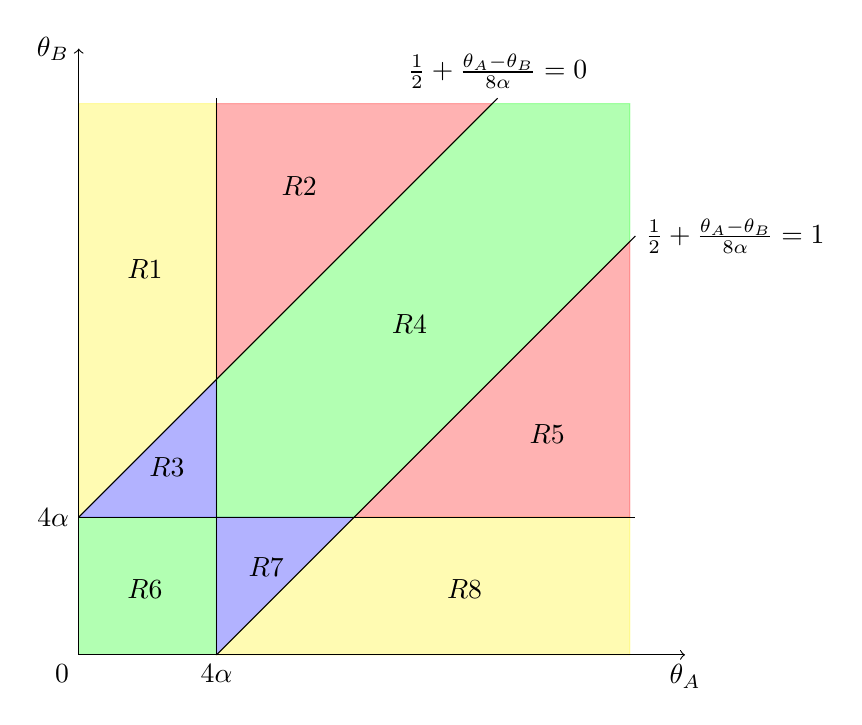
\begin{tikzpicture}[scale=7]
					%regions
					\filldraw[yellow, opacity=0.3] (0,1) -- (0,0.25) -- (0.25,0.5) |- (0,1);
					\filldraw[red, opacity=0.3] (0.25,0.5) -- (0.75,1) -| (0.25,0.5);
					\filldraw[blue, opacity=0.3] (0,0.25) -- (0.25,0.5) |- (0,0.25);
					\filldraw[green, opacity=0.3] (0.25,0.5) |- (0.5,0.25) -- (1,0.75) |- (0.75,1) --(0.25,0.5);
					\filldraw[red, opacity=0.3] (0.5,0.25) -- (1,0.75) |- (0.5,0.25);
					\filldraw[green, opacity=0.3] (0,0) -| (0.25,0.25) -| (0,0);
					\filldraw[blue, opacity=0.3] (0.25,0) -- (0.5,0.25) -| (0.25,0);
					\filldraw[yellow, opacity=0.3] (1,0) -- (0.25,0) -- (0.5,0.25) -| (1,0);
					\draw (0.12,0.7) node{$R1$};
					\draw (0.4,0.85) node{$R2$};
					\draw (0.16,0.34) node{$R3$};
					\draw (0.6,0.6) node{$R4$};
					\draw (0.85,0.4) node{$R5$};
					\draw (0.12,0.12) node{$R6$};
					\draw (0.34,0.16) node{$R7$};
					\draw (0.7,0.12) node{$R8$};
					
					% axes 
					\draw[->] (0,0) -- (1.1,0) node[below]{$\theta_A$};
					\draw[->] (0,0) -- (0,1.1) node[left]{$\theta_B$};
					\draw (0,0) node[below left]{$0$};
					\draw (0,0.25) -- (0.76,1.01) node[above]{$\frac{1}{2} + \frac{\theta_A - \theta_B}{8\alpha}=0$};
					\draw (0.25,0) -- (1.01,0.76) node[right]{$\frac{1}{2} + \frac{\theta_A - \theta_B}{8\alpha}=1$};
					\draw (0,0.25) -- (1.01,0.25);
					\draw (0.25,0) -- (0.25,1.01);
					\draw (0.25,0) node[below]{$4\alpha$};
					\draw (0,0.25) node[left]{$4\alpha$};
				\end{tikzpicture}
				\caption{regions of types for the cake problem.}
				\label{fig:cake}
			\end{center}
		\end{figure}
		
		\item Within the monetary realm, Dad can withhold kids' future allowance, which should be similar to requiring a payment. Alternatively, methods of payment can include cutting down on the kids' screen time (on a smartphone, tv, Nintendo Switch\texttrademark, etc), bedtime, curfew time, or similar. Symmetrically, transfers \emph{to} the kids can be implemented by increasing their respective time allowance.
		
		%\item The welfare-maximizing allocation rule $k^*(\theta)$ relies on the objective function (``social welfare'') not being a function of transfers -- i.e., regardless of the transfers required to implement $k^*(\theta)$, it remains optimal to do so. The question then can be paraphrased as: is the objective function that our mechanism aims to maximize specified correctly or should it also depend on transfers somehow?
		%
		%The answer to this question would depend on your answer to part 3 above and your thoughts on parenting. One argument could be that a simple desire to eat some cake should not cause any repercussions, hence Dad should look among mechanisms without transfers -- somehow characterize the set of allocation rules that are IC without transfers and somehow select the best among them. Another viewpoint could be that the instrument via which transfers are imposed is important to the kids (so it provides incentives) but not to Dad (so it can be excluded from the objective), so VCG is perfectly fine. Finally, one could make the argument that transfers are important to all parties, so they should enter Dad's objective function. In that case the optimal mechanisms machinery could be used to derive a mechanism that maximizes welfare while also maximizing (or minimizing) the sum of kids' transfers to the mechanism.
	\end{enumerate}
	\fi
	
	
	
	
	\section{Used Car Auction}
	% final2021_1. opt.mech, simple dynamics (no IRFs)
	Monica is running a used car auction. This week she has two cars for sale: a '85 Ford Mustang and an '87 Pontiac Trans Am, hereinafter denoted as $c \in \{F,P\}$. The auction has attracted $N$ interested bidders $i\in \{1,...,N\}$, whose valuations are commonly believed to be $\theta_{i,c} \sim \text{i.i.d.}U[0,1]$. In particular, for every $i$, $\theta_{i,F}$ is independent of $\theta_{i,P}$, since the two cars are quite different and have different age-related issues. However, once a bidder wins one car, they are not interested in bidding for another. Monica's value for retaining either car is $\bar{\theta} \in [0,1]$ and $2\bar{\theta}$ if she retains both. All players' preferences are Euclidean. Your goal is to help Monica design the auction in such a way as to generate the most revenue.
	
	\begin{enumerate}
		\item Suppose the cars are auctioned sequentially over two periods $t=1,2$, and at $t=2$ there are only one car $c=P$ and $N-1$ bidders left. Derive the optimal auction (for $t=2$) that maximizes Monica's expected revenue. Make sure to describe both the allocation and the payment rules.
		
		\item Calculate buyer $i$'s ex ante expected utility from participating in the auction you derived.
		
		\item Now move on to $t=1$ and the auction for $c=F$. Suppose that at this point the buyers do not yet know their valuations $\theta_{i,P}$ for the second car (since it has not yet been presented and they did not have a chance to inspect it). Derive the optimal auction for $c=F$ in $t=1$, assuming that in $t=2$ the auction for $c=P$ will be run according to the rules you derived in part 1.
		
		\item How do you think the expected revenue $R_F$ from selling $c=F$ in $t=1$ compares with the expected revenue from selling $c=P$ in $t=2$? (A convincing intuitive argument suffices.) What implications do your conclusions have for auction design? (I.e., is it optimal to sell the two items sequentially or could a different format yield better results?)
	\end{enumerate}
	
	
	
	\ifsolutions
	\subsection*{Solution}
	\begin{enumerate}
		\item Following the slides for the optimal auctions, we get that Monica's expected profit is given by
		\begin{gather}
			\begin{aligned} 
				\mathbb{E}U_{M,2} &= \mathbb{E}_\theta \left[ \sum_{i=1}^{N-1} t_{i,2}(\theta) - k_{i,2} \bar{\theta} \right]
				\\
				&= \mathbb{E}_\theta \left[ \sum_{i=1}^{N-1} \left(k_{i,2}(\theta) VS_{i,2}(\theta) - U_{i,2}(0,\theta_{-i,P})\right) \right],
				\label{eq:carauction}
			\end{aligned}
			\\
			\nonumber
			\begin{aligned} 
				\text{where } VS_{i,2}(\theta) &= \theta_{i,P} - \bar{\theta} - \frac{1-\Phi_i(\theta_{i,P})}{\phi_i(\theta_{i,P})}
				\\
				&= 2\theta_{i,P} - (1+\bar{\theta}).
			\end{aligned}
		\end{gather}
		Note that it is convenient to incorporate $\bar{\theta}$ directly in the objective function as a loss if a trade takes place. If we do this, we can include it in $VS$ as a part of the real surplus generated from trade, $\theta_{i,P} - \bar{\theta}$.
		
		At $t=2$, bidders' outside option is zero, hence the minimal $U_{i,2}(0,\theta_{i,P})$ we can set is zero for all $i,\theta_{i,P}$. Further, maximizing $\mathbb{E}U_{M,2}$ over allocation rules $k$ that are feasible ($\sum_{i=1}^{N-1}k_{i,2} \leq 1$), we get
		\begin{align*}
			k_{i,2}^*(\theta) = \begin{cases}
				1 & \text{ if } \theta_{i,P} \geq \hat{\theta}_{i,2},
				\\
				0 & \text{ otherwise},
			\end{cases}
		\end{align*}
		where $\hat{\theta}_{i,2} = \max \left\{\frac{1+\bar{\theta}}{2}, \max_{j \neq i} \{ \theta_{j,P} \} \right\}$ is the minimal winning report for $i$ given others' reports.
		We can see that this allocation rule is monotone (it needs to be increasing in $\theta_{i,P}$ in this problem) for all $\theta_{-i,P}$, hence it is implementable in dominant strategies. To find the transfers that support it, use the ERP for the bidders' utility: 
		\begin{align*}
			U_{i,2}(\theta_{i,P},\theta_{-i,P}) = \theta_{i,P} k_{i,2}(\theta) - t_{i,2}(\theta) &= U_{i,2}(0,\theta_{-i,P}) + \int_0^{\theta_{i,P}} k_{i,2}(\theta) d\theta_{i,P}
			\\
			&= \max \{ \theta_{i,P} - \hat{\theta}_{i,2}, 0 \}
			\\
			\Rightarrow t_{i,2}(\theta) &= \begin{cases}
				\hat{\theta}_{i,2} & \text{ if } \theta_{i,P} \geq \hat{\theta}_{i,2}
				\\
				0 & \text{ otherwise}.
			\end{cases}
		\end{align*}
		It is trivial to verify that the resulting mechanism is IR for all $i,\theta_{i,P},\theta_{-i,P}$.
		
		We conclude that the optimal auction at $t=2$ is a second-price auction with reserve price equal to $\frac{1+\bar{\theta}}{2}$. 
		
		\item We have calculated that $U_{i,2}(\theta) = \max \{ \theta_{i,P} - \hat{\theta}_{i,2}, 0 \}$, hence
		\begin{align*}
			\mathbb{E}_\theta U_{i,2}(\theta_i,\theta_{-i}) &= \int_0^1 \int_0^1 \max \{ \theta_{i,P} - \hat{\theta}_{i,2}, 0 \} d \Phi_i(\theta_{i,P}) d \hat{\Phi}_i (\hat{\theta}_{i,2}) 
			\\
			&= \int_0^1 \left[ \int_{\hat{\theta}_{i,2}}^1 (\theta_{i,P} - \hat{\theta}_{i,2}) d\theta_{i,P} \right] d \hat{\Phi}_i (\hat{\theta}_{i,2}) 
			\\
			&= \int_0^1 \left[ \frac{(1-\hat{\theta}_{i,2})^2}{2} \right] d \hat{\Phi}_i (\hat{\theta}_{i,2}),
		\end{align*}
		where $\hat{\Phi}_i (\cdot)$ is the cdf of $\hat{\theta}_{i,2}$:
		\begin{align*}
			\hat{\Phi}_i (\hat{\theta}_{i,2}) &= \mathbb{P} \left\{ \max \left\{\frac{1+\bar{\theta}}{2}, \max_{j \neq i} \{ \theta_{j,P} \} \right\} \leq \hat{\theta}_{i,2} \right\}
			\\
			& = \begin{cases}
				0 & \text{ if } \hat{\theta}_{i,2} < \frac{1+\bar{\theta}}{2}
				\\
				\mathbb{P} \left\{ \max_{j \neq i} \{ \theta_{j,P} \} \leq \hat{\theta}_{i,2} \right\} & \text{ if } \hat{\theta}_{i,2} \geq \frac{1+\bar{\theta}}{2}
			\end{cases}
			\quad 
			= \begin{cases}
				0 & \text{ if } \hat{\theta}_i < \frac{1+\bar{\theta}}{2}
				\\
				\hat{\theta}_{i,2}^{N-2} & \text{ if } \hat{\theta}_i \geq \frac{1+\bar{\theta}}{2}
			\end{cases}
		\end{align*}
		(recall that $\max_{j \neq i} \{ \theta_{j,P} \}$ is a max of $N-2$ elements, since it is assumed there is a total of $N-1$ bidders at this stage). So we have (for $\hat{\theta}_{i,2} \geq \frac{1-\bar{\theta}}{2}$) that $d \hat{\Phi}_i (\hat{\theta}_{i,2}) = \hat{\phi}_i(\hat{\theta}_{i,2}) d \hat{\theta}_{i,2} = (N-2) \hat{\theta}_{i,2}^{N-3} d \hat{\theta}_{i,2}$, and at $\hat{\theta}_{i,2}=\frac{1+\bar{\theta}}{2}$, $\hat{\Phi}_i(\hat{\theta}_{i,2})$ jumps up from zero to $\frac{1+\bar{\theta}}{2}$. Plugging this in, we get
		\begin{align}
			\mathbb{E}_\theta U_{i,2}(\theta_{i,P},\theta_{-i,P}) &= \left.\left( \frac{(1-\hat{\theta}_{i,2})^2}{2} \right) \right|_{\hat{\theta}_{i,2}=\frac{1+\bar{\theta}}{2}} \cdot \left[ \left(\frac{1+\bar{\theta}}{2}\right)^{N-2} - 0^{N-2} \right]
			+ \int_{\frac{1+\bar{\theta}}{2}}^1 \frac{(1-\hat{\theta}_{i,2})^2}{2} (N-2) \hat{\theta}_{i,2}^{N-3} d \hat{\theta}_{i,2}
			\nonumber
			\\
			&= \frac{1}{N} \left(\frac{1+\bar{\theta}}{2}\right)^N - \frac{1}{N-1} \left(\frac{1+\bar{\theta}}{2}\right)^{N-1} + \frac{1}{N(N-1)}
			\label{eq:cars_utilt2}
		\end{align}
		It can be verified (analytically or graphically) that this function is decreasing in $N$.
		
		\item The difference between the two periods is that at $t=1$, the bidders' outside option from not participating in the auction or not winning the item is not zero, since they have an option to participate at $t=2$, which yields positive expected utility. At the same time, if a bidder wins $F$ at $t=1$, they forego this value (since, as assumed in the problem, they have no value for a second car, and will not participate at $t=2$).
		Letting $\alpha$ denote the probability that Ford is sold at $t=1$ to one of the other $N-1$ bidders, \eqref{eq:cars_utilt2} implies the outside option is given by
		\begin{align*}
			%\bar{U} = \alpha \frac{1}{N} \left( 1 - \left(\frac{1+\bar{\theta}}{2}\right)^N \right) + (1-\alpha) \frac{1}{N+1} \left( 1 - \left(\frac{1+\bar{\theta}}{2}\right)^{N+1} \right).
			\bar{U} = \frac{1-\alpha}{N+1} \left(\frac{1+\bar{\theta}}{2}\right)^{N+1} + \frac{2\alpha - 1}{N} \left(\frac{1+\bar{\theta}}{2}\right)^N - \frac{\alpha}{N-1} \left(\frac{1+\bar{\theta}}{2}\right)^{N-1} + \frac{1-\alpha}{(N+1)N} + \frac{\alpha}{N(N-1)}.
			%\bar{U} = \frac{\alpha}{N(N-1)} \left[ (N-1)\left(\frac{1+\bar{\theta}}{2}\right)^N - N \left(\frac{1+\bar{\theta}}{2}\right)^{N-1} + 1 \right] + \frac{1-\alpha}{(N+1)N} \left[ N \left(\frac{1+\bar{\theta}}{2}\right)^{N+1} - (N+1) \left(\frac{1+\bar{\theta}}{2}\right)^Z + 1 \right]
		\end{align*}
		Bidder $i$'s utility function at $t=1$ is then given by $u_{i,1}(x,\theta) = \theta_{i,F} k_{i,1} + \bar{U}(1-k_{i,1}) - t_{i,1}$.
		All derivations leading to expression \eqref{eq:carauction} still apply in this case, with the virtual suprlus now being $$VS_{i,1}(\theta) = (\theta_{i,F}-\bar{U}) - \bar{\theta} - \frac{1-\Phi_i(\theta_{i,F})}{\phi_i(\theta_{i,F})} = 2\theta_{i,F} - (1+\bar{U}+\bar{\theta}).$$ 
		The optimal allocation rule is hence given by
		\begin{align*}
			k_{i,1}^*(\theta) = \begin{cases}
				1 & \text{ if } \theta_{i,F} \geq \hat{\theta}_{i,1}
				\\
				0 & \text{ otherwise}
			\end{cases},
		\end{align*}
		where $\hat{\theta}_{i,1} = \max \left\{\frac{1+\bar{U}+\bar{\theta}}{2}, \max_{j \neq i} \{ \theta_{j,F} \} \right\}$.
		However, now the lowest we can set $U_{i,1}(0,\theta_{-i,F})$ to is $U_{i,1}(0,\theta_{-i,F}) = \bar{U}$, implying that the transfers are given by
		\begin{align*}
			\theta_{i,F} k_{i,1} + \bar{U}(1-k_{i,1}) - t_{i,1} &= \bar{U} + \max \{ \theta_{i,F} - \hat{\theta}_{i,1}, 0 \}
			\\
			\Rightarrow t_{i,1}(\theta) &= \begin{cases}
				\hat{\theta}_{i,1} - \bar{U} & \text{ if } \theta_{i,F} \geq \hat{\theta}_{i,1}
				\\
				0 & \text{ otherwise}
			\end{cases}.
		\end{align*}
		Note that this is not the final solution: $k^*_{i,1}$ and $t_{i,1}$ both depend on $\hat{\theta}_{i,1}$, which depends on $\bar{U}$, which depends on $\alpha$, which depends on $k^*_1$, hence we have a closed system. Resolving this system yields the solution.
		
		\textbf{Remark:} the above adopts an intuitive assumption that entry to the second auction is unrestricted (which is plausible in this setting). However, this does not fully exploit the power of dynamic mechanisms. In particular, Monica could restrict access to the $t=2$ auction to only those agents who participate at $t=1$. This means the bidders' outside option $\bar{U}_n$ from dropping out of $t=1$ auction is then given by $\bar{U}_n = 0$, whereas continuing and not winning car $F$ yields $\bar{U}_p = \bar{U}$ as defined above (as long as all agents choose to participate in equilibrium). Asking all players to pay $\bar{U}_p - \bar{U}_n = \bar{U}$ in order to be admitted to the second-period auction could then serve as a free source of extra revenue. I.e., the optimal first-period mechanism if exclusion is possible consists of $k^*_{i,1}(\theta)$ defined above and 
		\begin{align*}
			t_{i,1}(\theta) &= \begin{cases}
				\hat{\theta}_{i,1} & \text{ if } \theta_{i,F} \geq \hat{\theta}_{i,1}
				\\
				\bar{U}_p & \text{ otherwise}
			\end{cases}.
		\end{align*}
		
		
		\item We can see that at $t=1$, the item is sold less frequently (since the winner's valuation now must be above $\frac{1+\bar{U}+\bar{\theta}}{2}$, as opposed to the $\frac{1+\bar{\theta}}{2}$ cutoff at $t=2$), and all bidders shade their bids (the winner pays the second-highest valuation minus $\bar{U}$). These two factors suggest that the expected revenue in $t=1$ will be lower. However, there is another factor, which is that the competition is more intense, since we have $N$ bidders for sure at $t=1$ and we may have $N-1$ bidders at $t=2$. This effect may dominate for small $N$, leading to higher revenue at $t=1$. 
		
		Either way, the total revenue from both periods would be lower than if the bidders did not about the existence of both cars from the start. So it might be optimal to announce an auction for $c=F$, sell that via an SPA with reserve $\frac{1+\bar{\theta}}{2}$, and then announce that $c=P$ is also for sale in another similar SPA. However, that may attract fewer interested bidders $N$ to start with, reducing the revenue again. In the end, the solution is not clear-cut without further calculations and assumptions about bidder participation.
	\end{enumerate}
	\fi
	
	
	
	
	
	
	
	%%-----------------------------------------------------------------------------------------------------
	
\end{document}
